% ------------------------------------------------------------------------------
% TYPO3 Version 10.2 - What's New (Dutch Version)
%
% @license	Creative Commons BY-NC-SA 3.0
% @link		http://typo3.org/download/release-notes/whats-new/
% @language	Dutch
% ------------------------------------------------------------------------------

\section{Gebruikersinterface backend}
\begin{frame}[fragile]
	\frametitle{Gebruikersinterface backend}

	\begin{center}\huge{Hoofdstuk 1:}\end{center}
	\begin{center}\huge{\color{typo3darkgrey}\textbf{Gebruikersinterface backend}}\end{center}

\end{frame}

% ------------------------------------------------------------------------------
% Feature | 89458 | Show link to online docs in extension manager

\begin{frame}[fragile]
	\frametitle{Gebruikersinterface backend}
	\framesubtitle{Extensie Manager}

	De module Extensies toont nu links naar de documentatie van de extensie.

	\begin{figure}
		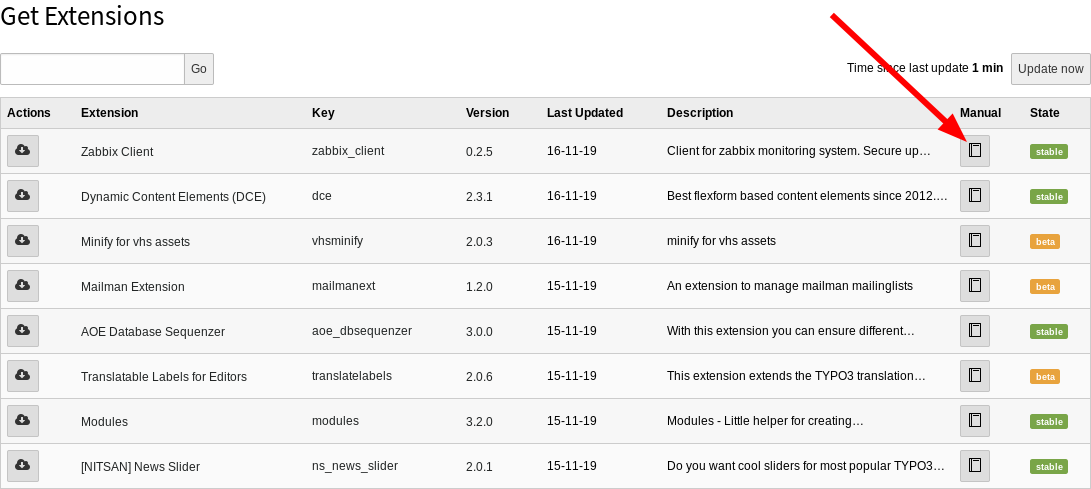
\includegraphics[width=0.90\linewidth]{ChangesForIntegrators/89458-ShowLinkToOnlineDocsInExtensionManager.png}
	\end{figure}

\end{frame}

% ------------------------------------------------------------------------------
% Feature | 86818 | Reintroduce keyboard accessible version of the pagetree

\begin{frame}[fragile]
	\frametitle{Gebruikersinterface backend}
	\framesubtitle{Toegankelijkheid paginaboom}

	Backend gebruikers kunnen nu hun toetsenbord gebruiken om te navigeren door de paginaboom.
	Toetsen die gebruikt kunnen worden zijn bijvoorbeeld de pijltjestoetsen, "home", "end", "enter", "space", etc.
	\newline
	Dit is gebaseerd op de adviezen die door de W3C zijn opgesteld in
	\href{https://www.w3.org/TR/wai-aria-practices-1.1/#keyboard-interaction-22}{WAI-ARIA Authoring Practices 1.1}.

	\begin{figure}
		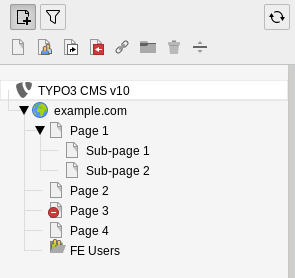
\includegraphics[width=0.30\linewidth]{BackendUserInterface/86818-PagetreeAccessibility.png}
	\end{figure}

\end{frame}

% ------------------------------------------------------------------------------
